% !TEX encoding = UTF-8 Unicode 
%
% Use:
% magister / inzynier - for master thesis or engineering thesis
% druk / archiwum - for print version or archive version
% en - to translate template into english
% examples:
%\documentclass[inzynier,druk,en] - master thesis, print version, english
%\documentclass[magister,druk,en]{dyplom}
%\documentclass[magister,druk]{dyplom}

\documentclass[inzynier,druk]{dyplom}

\usepackage{multicol}
\usepackage{minted}
\usepackage{pdflscape}
\usepackage{graphicx}
\usepackage{float}
\usepackage{subcaption}
\usepackage{amsmath}
\usepackage{amsfonts}

\usepackage[utf8]{inputenc}
\usepackage{hyperref}

% Maximum section's depth.
\setcounter{secnumdepth}{4}

% Listings settings
\setminted{breaklines, 
frame=lines,           
framesep=3mm,          
baselinestretch=1.1,   
fontsize=\small,       
% linenos              % line numbering
}

\usepackage{lipsum}

\faculty{Wydział informatyki i Telekomunikacji}                   % Uncomment if applicable
\fieldofstudy{Cyberbezpieczeńśtwo (CBE)}                          
\author{Patryk Fidler}
\title{Zastosowanie dużych modeli językowych do wykrywania i naprawiania błędów bezpieczeństwa i podatności w kodzie aplikacji webowych}
\supervisor{Dr. hab. inż. Maciej Piasecki}
% \consultant{Consultant's name}               % Uncomment if applicable
\specialisation{Bezpieczeństwo danych (CBD)}                         % Uncomment if applicable
\keywords{modele językowe, Sztuczna Inteligencja, statyczna analiza kodu}	% 3-5 keywords  

\begin{document}
\maketitle

\abstract{
% Polish abstract 
Praca inżynierska zatytułowana "Zastosowanie dużych modeli językowych do wykrywania i naprawiania błędów bezpieczeństwa i podatności w kodzie aplikacji webowych" koncentruje się na zastosowaniu zaawansowanych modeli językowych, takich jak GPT-3.5, GPT-4, a w przyszłości także modele otwartoźródłowe, takie jak Mistral, do automatycznego wykrywania i naprawiania błędów bezpieczeństwa w kodzie oprogramowania i aplikacji webowych.

Motywacja tej pracy wynika z rosnącej roli dużych modeli językowych (LLM) w różnych dziedzinach, w tym w cyberbezpieczeństwie. W kontekście tych działań, badana jest możliwość wykorzystania tych modeli do wykrywania i naprawiania podatności takich jak XSS, SQL Injection, CSRF, Buffer Overflow i tym podobne.

Punktem wyjścia dla pracy dyplomowej jest artykuł napisany w 2021 roku 
"Can OpenAI Codex and Other Large Language Models Help Us Fix Security Bugs?"
- Hammond Pearce, Benjamin Tan, Baleegh Ahmad, Ramesh Karri, Brendan Dolan-Gavitt (https://arxiv.org/pdf/2112.02125v1.pdf). Autorzy podkreślają znaczący potencjał tych modeli, a niniejsza praca ma na celu kontynuację tych badań i poszerzenie ich zakresu.

Planowane działania obejmują przygotowanie zbioru danych zawierającego podatne bazy kodu źródłowego, testowanie zdolności detekcji błędów przez modele językowe OpenAI, oraz porównanie tych wyników z istniejącymi rozwiązaniami, oferowanymi przez firmę Snyk. 

Szczególny nacisk zostanie położony na wykorzystanie technik uczenia się w kontekście (in-context learning) oraz generowanie wspomagane pobieraniem (RAG - Retrieval Augmented Generation), które mogą pomóc w udoskonaleniu detekcji i wyników, nawet przy ograniczonych zasobach. 
Praca przewiduje implementację autonomicznego agenta AI zdolnego do analizy kodu, wykonania testów bezpieczeństwa i podejmowania decyzji na podstawie wyników tych testów i kontekstu.

Opcjonalnie, badane będą możliwości detekcji błędów przez otwarte modele językowe, a w dalszej perspektywie, możliwości specjalizacji modeli w zakresie cyberbezpieczeństwa za pomocą fine-tuning'u. Wszystkie te działania mają na celu nie tylko badanie, ale także poprawienie możliwości LLM w kontekście cyberbezpieczeństwa.

Głównym celem pracy jest zwiększenie świadomości na temat potencjału dużych modeli językowych w cyberbezpieczeństwie oraz proponowanie praktycznych rozwiązań, które mogą pomóc programistom w tworzeniu bardziej bezpiecznych aplikacji.

}{
% Abstract translated into English
The engineering thesis titled "Application of Large Language Models for Detecting and Fixing Security Bugs and Vulnerabilities in Web Application Code" focuses on the utilization of advanced language models, such as GPT-3.5, GPT-4, and if possible, Falcon, for automated detection and rectification of security bugs in the code of software and web applications.

The motivation for this work stems from the growing role of Large Language Models (LLMs) in various fields, including cybersecurity. In the context of these efforts, the possibility of using these models to detect and fix vulnerabilities such as XSS, SQL Injection, CSRF, Buffer Overflow, and the like is being investigated.

The starting point for this dissertation is the 2021 article "Can OpenAI Codex and Other Large Language Models Help Us Fix Security Bugs?" by Hammond Pearce, Benjamin Tan, Baleegh Ahmad, Ramesh Karri, Brendan Dolan-Gavitt (https://arxiv.org/pdf/2112.02125v1.pdf). The authors emphasize the significant potential of these models, and this work aims to continue this research and broaden its scope.

Planned activities include preparing a dataset containing vulnerable source code databases, testing the error detection capabilities of OpenAI language models, and comparing these results with existing solutions offered by Snyk.

Particular emphasis will be placed on the use of soft-prompting and in-context learning techniques, which can help improve detection and results, even with limited resources. The work also envisages the implementation of an autonomous AI agent capable of analyzing code, performing security tests, and making decisions based on the results of these tests and context.

Optionally, the possibilities of error detection by open language models will be explored, and in the longer term, the possibilities of specializing models in the field of cybersecurity through fine-tuning. All these actions aim not only to understand but also to improve the capabilities of LLMs in the context of cybersecurity.

The main goal of the work is to increase awareness of the potential of large language models in cybersecurity and to propose practical solutions that can help developers create more secure applications.

}

\tableofcontents

% !TEX encoding = UTF-8 Unicode 
% !TEX root = praca.tex


\chapter*{Wprowadzenie}

Niniejsza praca inżynierska nosi tytuł "Zastosowanie dużych modeli językowych do wykrywania i naprawiania błędów bezpieczeństwa i podatności w kodzie aplikacji webowych". Celem tej pracy jest zbadanie, w jaki sposób zaawansowane modele językowe, takie jak GPT-3.5, GPT-4 oraz modele otwarto-źródłowe - Mistral 7B, Falcon-7B-instruct, mogą być wykorzystane do automatycznego wykrywania i naprawiania błędów bezpieczeństwa w kodzie oprogramowania i aplikacji webowych. 
W tym celu zostanie opracowane i zaimplementowane narzędzie do statycznej analizy kodu, które będzie wykorzystywać modele językowe do generowania kodu i naprawy błędów.
Narzędzie to zostanie przetestowane i porównane z innymi rozwiązaniami, takimi jak Snyk, które oferują podobne funkcjonalności.
W pracy zostaną przedstawione wyniki badań, które mają na celu odpowiedzieć na pytanie, czy modele językowe mogą być wykorzystane do tego celu, oraz jak skuteczne są one w porównaniu z innymi rozwiązaniami.
W ramach pracy zostaną również zbadane ograniczenia i wyzwania związane z wykorzystaniem tych technologii w kontekście cyberbezpieczeństwa.

\section*{Pytania badawcze}
W ramach pracy stawiam następujące pytania badawcze:
\begin{enumerate}
    \item Czy duże modele językowe mogą być wykorzystane do wykrywania i naprawiania błędów bezpieczeństwa w kodzie aplikacji webowych?
    \item Jak skuteczne są te modele w porównaniu z innymi rozwiązaniami?
    \item Czy komercyjne modele językowe znacznie różnią się od otwartych modeli?
    \item Jakie są ograniczenia i wyzwania związane z wykorzystaniem tych technologii w kontekście cyberbezpieczeństwa?
\end{enumerate}

\section*{Hipotezy}
Hipotezy pracy to:
\begin{enumerate}
    \item Duże modele językowe, dzięki swojej zdolności do analizy i generowania kodu, mogą skutecznie identyfikować i naprawiać błędy bezpieczeństwa w kodzie źródłowym.
    \item Mimo obiecującego potencjału, modele te mogą napotykać ograniczenia, szczególnie w bardziej złożonych i specyficznych scenariuszach związanych z cyberbezpieczeństwem.
\end{enumerate}

\section*{Uzasadnienie tytułu}
Tytuł pracy został dobrany tak, aby odzwierciedlał główny obszar zainteresowania badawczego, jakim jest wykorzystanie nowoczesnych technologii językowych w celu poprawy bezpieczeństwa aplikacji webowych. 
W kontekście rosnącej zależności od cyfrowych rozwiązań, temat ten zyskuje na znaczeniu, oferując nowe perspektywy i podejścia do zagadnień bezpieczeństwa.
Tytuł można skrócić do \textbf{''Zastosowanie dużych modeli językowych w statycznej analizie kodu''}, ponieważ tak nazywa się problem odnajdywania i korekcji błędów w kodzie źródłowym. 
Korpus badawczy pracy został rozszerzony o projekty open-source aplikacji natywnych i desktopowych oraz wycinki błędnego kodu i poprawnego kodu. 

\section*{Omówienie literatury naukowej i stopnia jej przydatności}
Podstawę teoretyczną pracy stanowi literatura naukowa skupiająca się na dużych modelach językowych oraz ich zastosowaniu w cyberbezpieczeństwie. Szczególną uwagę poświęcono artykułowi ''Can OpenAI Codex and Other Large Language Models Help Us Fix Security Bugs?'', który posłużył jako punkt wyjścia dla badań. 
Praca ta ma na celu kontynuację i poszerzenie zakresu tych badań, wykorzystując literaturę naukową jako fundament do eksploracji nowych możliwości w zakresie analizy i naprawy błędów w kodzie.
Różnica między pracą a literaturą naukową polega na tym, że praca skupia się na praktycznym zastosowaniu modeli językowych w celu wykrywania i naprawiania błędów bezpieczeństwa w kodzie, podczas gdy literatura naukowa skupia się na badaniu możliwości Sztucznej Inteligencji w tym zakresie.

\section*{Cel pracy}
Głównym celem pracy jest zbadanie możliwości wykorzystania dużych modeli językowych do wykrywania i naprawiania błędów bezpieczeństwa i podatności w kodzie źródłowym aplikacji webowych. 
W tym kontekście można wyróżnić następujące cele pośrednie:
\begin{itemize}
    \item Opracowanie praktycznego rozwiązania do statycznej analizy kodu dla aplikacji webowych oraz lokalnych.
    \item Badanie skuteczności dużych modeli językowych w wykrywaniu podatności i luk bezpieczeństwa.
\end{itemize}

\section*{Zakres pracy}
Zakres pracy obejmuje:
\begin{itemize}
    \item Analizę istniejącej literatury i badań, w szczególności artykułu 'Can OpenAI Codex and Other Large Language Models Help Us Fix Security Bugs?'.
    \item Projektowanie i implementacja narzędzia do statycznej analizy kodu opartego na modelach OpenAI.
    \item Przygotowanie zbioru danych z kodem zawierającym potencjalne podatności.
    \item Testowanie i porównanie skuteczności z innymi rozwiązaniami, np. oferowanymi przez firmę Snyk.
    \item Analiza wyników i formułowanie wniosków.
\end{itemize}


\addcontentsline{toc}{chapter}{Analiza istniejącej literatury oraz dotychczasowych badań}
\chapter{Analiza istniejącej literatury oraz dotychczasowych badań}

\section{Can OpenAI Codex and Other Large Language Models Help Us Fix Security Bugs?}
% https://arxiv.org/pdf/2112.02125v1.pdf

\subsection{Metodologia}
W badaniu "Czy OpenAI Codex i inne duże modele językowe mogą pomóc nam naprawić błędy bezpieczeństwa?", autorzy skupili się na wykorzystaniu dużych modeli językowych (LLM) do naprawy podatności w kodzie w sposób zero-shot. Badanie koncentrowało się na projektowaniu monitów skłaniających LLM do generowania poprawionych wersji niebezpiecznego kodu. Przeprowadzono eksperymenty na szeroką skalę, obejmujące różne komercyjne modele LLM oraz lokalnie wytrenowany model.

\subsection{Wyniki}
Wyniki wykazały, że LLM mogą skutecznie naprawić 100\% syntetycznie wygenerowanych scenariuszy oraz 58\% podatności w historycznych błędach rzeczywistych projektów open-source. Odkryto, że różne sposoby formułowania informacji kluczowych w monitach wpływają na wyniki generowane przez modele. Zauważono, że wyższe temperatury generowania kodu przynoszą lepsze wyniki dla niektórych typów podatności, ale gorsze dla innych.

\section{Examining Zero-Shot Vulnerability Repair with Large Language Models}
% https://arxiv.org/pdf/2112.02125.pdf

W artykule "Examining Zero-Shot Vulnerability Repair with Large Language Models", autorzy kontynuowali badanie możliwości wykorzystania LLM do naprawy podatności w kodzie, koncentrując się na wyzwaniach związanych z generowaniem funkcjonalnie poprawnego kodu w rzeczywistych scenariuszach. Badanie to rozszerzało wcześniejsze prace, biorąc pod uwagę bardziej złożone przypadki użycia LLM.

Podstawowe pytania badawcze były następujące:
\begin{enumerate}
    \item Czy LLM mogą generować bezpieczny i funkcjonalny kod do naprawy podatności?
    \item Czy zmiana kontekstu w komentarzach wpływa na zdolność LLM do sugerowania poprawek?
    \item Jakie są wyzwania przy używaniu LLM do naprawy podatności w rzeczywistym świecie?
    \item Jak niezawodne są LLM w generowaniu napraw?
\end{enumerate}

Eksperymenty potwierdziły, że choć LLM wykazują potencjał, ich zdolność do generowania funkcjonalnych napraw w rzeczywistych warunkach jest ograniczona. Wyzwania związane z inżynierią promptów i ograniczenia modeli wskazują na potrzebę dalszych badań i rozwoju w tej dziedzinie.

\section{Różnice między obecną pracą a istniejącą literaturą}

W przeciwieństwie do dotychczasowych badań skoncentrowanych głównie na teoretycznym potencjale dużych modeli językowych (LLM) w kontekście zero-shot, niniejsza praca dyplomowa podejmuje kroki w kierunku praktycznego zastosowania tych technologii. Główną różnicą jest tutaj zastosowanie metod takich jak Retrieval Augmented Generation (RAG) oraz in-context learning, co przesuwa nasze podejście w stronę kontekstu few-shot. 

\begin{itemize}
    \item \textbf{Zastosowanie Metod RAG i In-context Learning:} W odróżnieniu od tradycyjnych podejść zero-shot, które polegają na generowaniu odpowiedzi bez uprzedniego dostosowania modelu do specyficznego zadania, moja praca wykorzystuje RAG i uczenie się w kontekście, aby lepiej dostosować modele do konkretnych scenariuszy związanych z bezpieczeństwem kodu. Te metody pozwalają na bardziej precyzyjną analizę i naprawę błędów w kodzie.
    
    \item \textbf{Praktyczne Zastosowanie Modeli Językowych:} Podczas gdy większość istniejących badań skupia się na badaniu możliwości SI w teorii, ta praca koncentruje się na praktycznym zastosowaniu modeli językowych do wykrywania i naprawiania błędów bezpieczeństwa w kodzie. Przez to podejście, praca ta dostarcza bezpośrednich, aplikatywnych rozwiązań, które mogą być wykorzystane w rzeczywistych środowiskach programistycznych.
\end{itemize}

Takie podejście pozwala nie tylko na zrozumienie teoretycznego potencjału LLM, ale także na ocenę ich praktycznej przydatności w realnych scenariuszach związanych z cyberbezpieczeństwem. Znacząco poszerza to zakres badań w dziedzinie wykorzystania sztucznej inteligencji do poprawy bezpieczeństwa aplikacji, dostarczając nowych perspektyw i rozwiązań.

\chapter{Metodyka rozwiązania}

W niniejszej pracy dyplomowej zastosowano szereg metod i środków, aby zaimplementować narzędzie do statycznej analizy kodu oraz zbadać i ocenić potencjał dużych modeli językowych w kontekście wykrywania i naprawiania błędów bezpieczeństwa w kodzie źródłowym aplikacji.

\begin{table}[H]
    \begin{adjustwidth}{-2cm}{-2cm}  % Zmniejszenie marginesów z obu stron
        \centering
    \begin{tabular}{|>{\bfseries}p{2.5cm}|p{5cm}|>{\bfseries}p{2.5cm}|p{5cm}|}
    \hline
    \multicolumn{4}{|c|}{\textbf{Metody i Środki}} \\
    \hline
    \textbf{Metoda} & \small{Opis} & \textbf{Środek} & \small{Opis} \\
    \hline
    \textbf{Zero-shot learning} & \small{Metoda uczenia maszynowego pozwalająca modelom wykonywać zadania bez wcześniejszego treningu, opierając się na zdolności do rozumienia i generalizacji.} & \textbf{Modele językowe GPT-3.5, GPT-4} & \small{Zaawansowane modele AI OpenAI do generowania tekstu i odpowiadania na zapytania.} \\
    \hline
    \textbf{Prompt engineering} & \small{Projektowanie promptów w celu uzyskania trafnych odpowiedzi od AI.} & \textbf{OpenAI Assistant API} & \small{API umożliwiające integrację modeli językowych w aplikacjach.} \\
    \hline
    \textbf{In-context learning} & \small{Uczenie się i dostosowywanie modeli AI na podstawie informacji z promptów.} & \textbf{Zbiory danych z kodem} & \small{Zestawy danych z przykładami kodu zawierającymi błędy, używane do trenowania narzędzi do wykrywania podatności.} \\
    \hline
    \textbf{Retrieval Augmented Generation} & \small{Technika łącząca generowanie treści z wyszukiwaniem informacji, wspomagana przez OpenAI Assistant API.} & \textbf{Projekty open-source zawierające błędy bezpieczeństwa} & \small{Publiczne projekty mogące zawierać błędy bezpieczeństwa, używane do edukacji.} \\
    \hline
    \textbf{Analiza porównawcza} & \small{Ocena różnych technik lub systemów poprzez porównanie.} & \textbf{Statyczne testy podatności} & \small{Narzędzia analizy statycznej kodu, np. CodeQL.} \\
    \hline
    \textbf{Programowanie obiektowe i funkcyjne} & \small{Dwa paradygmaty programowania, koncentrujące się odpowiednio na obiektach i funkcjach.} & \textbf{Rozwiązania komercyjne, np. Snyk} & \small{Narzędzia AI do zarządzania bezpieczeństwem oprogramowania.} \\
    \hline
    & & \textbf{Python 3.12} & \small{Najnowsza wersja języka Python z zaawansowanymi funkcjami.} \\
    \hline
    & & \textbf{Biblioteki: openai, asyncio} & \small{Biblioteki Pythona dla integracji z OpenAI i programowania asynchronicznego.} \\
    \hline
    & & \textbf{Komputer osobisty} & \small{Urządzenie do tworzenia i testowania oprogramowania.} \\
    \hline
    \end{tabular}
\end{adjustwidth}
    \caption{Metody i środki wykorzystane w projekcie i badaniu.}
    \label{tab:methods_tools}
\end{table}

    

Metody i środki te zostały wybrane, aby zapewnić efektywne i wszechstronne podejście do analizy i naprawy kodu. Generacja wspomagana pobieraniem danych (RAG ang. Retrieval Augmented Generation) 
oraz uczenie się w kontekście(in-context learning) umożliwiają efektywną analizę i generowanie kodu. 
Z kolei analiza porównawcza pozwala na ocenę skuteczności różnych modeli i podejść. 
Wykorzystanie modeli językowych GPT-3.5 i GPT-4, środowiska Ollama, oraz innych narzędzi i zasobów, zapewnia solidną bazę do przeprowadzenia kompleksowych testów i analiz.



% !TEX encoding = UTF-8 Unicode 
% !TEX root = praca.tex

\chapter{Projektowanie i implementacja rozwiązania}

W ramach pracy dyplomowej opracowano aplikację \texttt{gptester}, , której celem jest statyczna analiza kodu w poszukiwaniu podatności bezpiec
zeństwa oraz proponowanie ich napraw. Aplikacja wykorzystuje modele GPT-4, lub GPT-3.5 dostarczane przez OpenAI i jest zaprojektowana do działania z linii komend, z wynikami zapisywanymi w pliku markdown.

\section{Opis rozwiązania}

Program \texttt{gptester}
jest narzędziem do statycznej analizy kodu, które korzysta z modelu GPT-4 do generowania raportów dotyczących jakości kodu i proponowania napraw. Głównym celem programu jest bezpieczeństwo kodu, które ma być w przyszłości rozszerzone. Aplikacja została napisana w języku Python, a model GPT-4 jest dostarczany przez OpenAI. Program jest przeznaczony do uruchamiania z linii poleceń, a wyniki są zapisywane w pliku markdown. Program można uruchomić z następującymi argumentami:

\begin{verbatim}

    ./main.py -h
    usage: main.py [-h] [--model MODEL] [--input INPUT] [--output OUTPUT]
\end{verbatim}

\begin{figure}
    \centering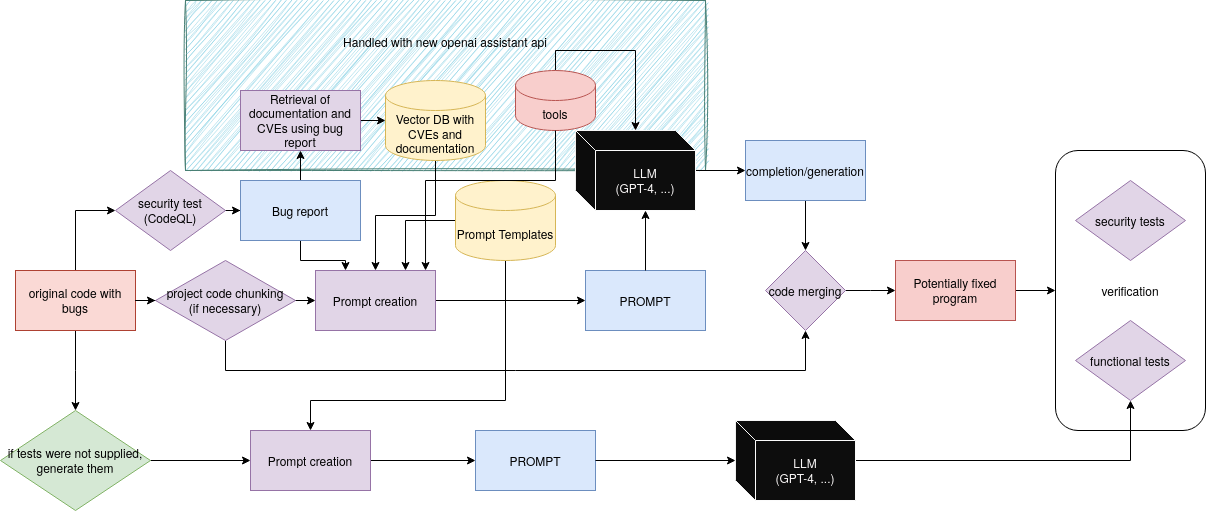
\includegraphics[width=.6\textwidth]{img/gptester.drawio.png}
    \caption{Schemat blokowy działania aplikacji}  \label{rys:schemat}
    \end{figure}
    
    Na rysunku \ref{rys:schemat} \dots
\chapter{Zbiory danych i ich przygotowanie}
\label{ch:zbiory_danych}

W kontekście niniejszego rozdziału dokonano prezentacji oraz analizy zbiorów danych, które zostały wykorzystane w procesie testowania programu \textbf{gptester} oraz badania skuteczności dużych modeli językowych (LLM). Szczegółowo opisany został proces przygotowania i przetwarzania tych zbiorów danych, co ma kluczowe znaczenie dla efektywności analizy statycznej kodu i kalibracji narzędzia.


\section{Przegląd wykorzystanych zbiorów danych}
\label{sec:przeglad_zbiorow}

Następująca sekcja zawiera omówienie źródeł danych, ich specyfikacji oraz roli, jaką odgrywają w kontekście projektu. Analiza ta obejmuje zarówno repozytoria kodu, jak i bazy danych przykładowych podatności.

\begin{itemize}
    \item \textbf{snoopysecurity/Vulnerable-Code-Snippets}: Repozytorium w serwisie Github zawierające zbiór fragmentów kodu zawierających luki bezpieczeństwa. Fragmenty pobrane z różnych wpisów na blogach, książek, zasobów itp. 
    Zbiór w głównej mierze używany do testowania implementacji. Niektóre fragmenty kodu zawierają wskazówki w nazwach/komentarzach. Ewentualne naruszenie praw autorskich niezamierzone.\\ \url{https://github.com/snoopysecurity/Vulnerable-Code-Snippets}

    % \item \textbf{DiverseVul}: \url{https://arxiv.org/abs/2304.00409} Opis kolejnego zbioru danych, jego charakterystyka i zastosowanie w kontekście `gptester`.
    % \item \textbf{CVEfixes}: \url{https://github.com/secureIT-project/CVEfixes}

    % \item \textbf{OWASP VulnerableApp}: Aplikacja webowa zawierająca szereg podatności, służąca do testowania narzędzi do analizy bezpieczeństwa aplikacji webowych. Napisana w języku PHP, kod źródłowy dostępny w repozytorium umożliwia pobranie obrazu kontenera Docker. \url{https://github.com/SasanLabs/VulnerableApp}

    % \item \textbf{Damn Vulnerable NodeJS Application (DVNA)}: Aplikacja napisana w NodeJS, demonstrująca podatności z TOP 10 OWASP, służąca do nauki i testowania narzędzi do analizy bezpieczeństwa aplikacji. Repozytorium zawiera instrukcje uruchomienia i testowania aplikacji. \url{https://github.com/appsecco/dvna}
    \item \textbf{OWASP/NodeGoat}: Repozytorium zawierające aplikację webową, która została stworzona w celu demonstracji podatności z TOP 10 OWASP. Aplikacja została napisana w NodeJS, a jej kod źródłowy jest dostępny w serwisie Github.\\ \url{https://github.com/OWASP/NodeGoat}

\end{itemize}

\section{Proces przygotowania danych}
\label{sec:proces_przygotowania_danych}

Dobrane przeze mnie zbiory danych zostały tak, by nie trzeba było dostosowywać programu do konkretnego formatu. Oznacza to, że wskazane repozytoria zawierają przykłady kodu zapisane w plikach.

\subsection{snoopysecurity/Vulnerable-Code-Snippets} 
Repozytorium zawiera wiele plików z przykładami kodu, które mogą zawierać błędy bezpieczeństwa. Pliki te zostały pobrane z różnych źródeł, takich jak blogi, książki, zasoby itp. Pliki te zawierają często komentarze lub nazwy zmiennych, które wskazują na potencjalne błędy bezpieczeństwa. Pozwala to nam na izolację problemu identyfikacji podatności od zadania generowania kodu. W pierwszej kolejności badania zostały przeprowadzone bez wprowadzania zmian w kodzie, aby ocenić skuteczność modeli językowych w korekcji błędów bezpieczeństwa. W kolejnym kroku, w celu przebadania zdolności do identyfikowania błędów, zostały wprowadzone zmiany w kodzie, takie jak usunięcie komentarzy, zmienienie nazw katalogów, plików i zmiennych. W ten sposób można było sprawdzić, czy modele językowe są w stanie wykryć błędy bezpieczeństwa, gdy mają różną ilość informacji na temat kodu.


% \subsection{OWASP VulnerableApp}
% Jako pełnoprawna aplikacja webowa, VulnerableApp pozwala na testowanie narzędzia `gptester` w realistycznym środowisku, z prawdziwymi podatnościami. Użycie tej aplikacji w badaniach pozwoliło na weryfikację skuteczności modeli językowych w wykrywaniu błędów bezpieczeństwa.

\subsection{OWASP/NodeGoat}
NodeGoat, jako aplikacja demonstrująca podatności OWASP Top 10, stanowiła cenne źródło do testowania `gptester`. Dzięki dokumentacji i instrukcjom dostępnym w repozytorium, możliwe było efektywne wykorzystanie tej aplikacji do celów badawczych.

\section{Wyzwania i ograniczenia}
\label{sec:wyzwania_i_ograniczenia}

Głównym wyzwaniem prezentowanym przez użyte przeze mnie próbki badawcze wynikają z ich charakteru. Zbiór danych Vulnerable-Code-Snippets nie jest reprezentatywne dla rzeczywistych aplikacji, a jedynie zawiera przykłady kodu, które mogą zawierać błędy bezpieczeństwa. W przypadku większości przykładów kodu, nie jest możliwe uruchomienie go bez posiadania kodu całego projektu, co utrudnia ewaluację. W związku z powyższym niektóre skrawki kodu zostały obudowane w aplikacje webową, natomiast inne pominięte. Nie każdy skrawek kodu w repozytorium jest wycięty z aplikacji webowej, te przykłady zostały uwzględnione w badaniach i sprawiały najmniej problemów. 

W kontekście OWASP NodeGoat, aplikacja ta była w pełni funkcjonalna i umożliwiała realistyczne testowanie podatności. Jednakże, wyzwaniem okazało się wykorzystanie wczesnej wersji \texttt{gptester}, która nie posiadała jeszcze możliwości aktualizacji bazy kodu przez systemy kontroli wersji. To z kolei wymuszało ręczne łączenie zmian w kodzie z nowymi wersjami aplikacji, co było procesem czasochłonnym i komplikowało przeprowadzenie badań. Testy bezpieczeństwa przeprowadzone przy użyciu skanerów podatności, zwłaszcza OWASP ZAP - zoptymalizowanego do wykrywania podatności w aplikacjach takich jak NodeGoat - miały za zadanie ocenić skuteczność proponowanych przez \texttt{gptester} korekt.


\section{Podsumowanie}

W rozdziale \ref{ch:zbiory_danych} przedstawiono i dokładnie przeanalizowano zbiory danych wykorzystane w badaniach nad skutecznością dużych modeli językowych (LLM) za pomocą programu \textbf{gptester}. Kluczowe znaczenie miało tutaj szczegółowe przygotowanie i przetwarzanie tych zbiorów, co miało bezpośredni wpływ na efektywność analizy statycznej kodu oraz kalibrację narzędzia.

Repozytorium \textit{snoopysecurity/Vulnerable-Code-Snippets} dostarczyło przykłady kodu zawierające potencjalne luki bezpieczeństwa, które umożliwiły testowanie zdolności \textbf{gptester} do identyfikacji i sugerowania napraw błędów bezpieczeństwa. Z kolei aplikacja \textit{OWASP/NodeGoat}, demonstrująca podatności z listy OWASP Top 10, posłużyła jako realistyczne środowisko do testowania skuteczności LLM w wykrywaniu podatności.

Wyzwaniem okazała się natura wykorzystanych próbek kodu, które często nie były reprezentatywne dla rzeczywistych aplikacji i wymagały dodatkowej pracy, aby mogły być użyte w testach. Wczesna wersja \textbf{gptester} również nałożyła ograniczenia na proces badawczy, szczególnie w kontekście aktualizacji bazy kodu i ręcznego scalania zmian.

Pomimo tych wyzwań, analiza zbiorów danych pozwoliła na zgłębienie możliwości i ograniczeń LLM w kontekście analizy bezpieczeństwa aplikacji webowych. Przeprowadzone badania podkreśliły znaczenie interdyscyplinarnego podejścia łączącego technologie LLM z wiedzą ekspercką w dziedzinie bezpieczeństwa, aby maksymalizować efektywność narzędzi typu \textbf{gptester} w wykrywaniu i naprawianiu podatności w oprogramowaniu.


% !TEX encoding = UTF-8 Unicode 
% !TEX root = praca.tex


\section*{Podsumowanie}
W pracy zbadano wykorzystanie dużych modeli językowych (LLM) w kontekście statycznej analizy kodu, skupiając się na ich zdolnościach do identyfikacji i naprawy błędów programistycznych. Rozpatrzono różne aspekty stosowania LLM, w tym ich integrację z istniejącymi narzędziami do analizy kodu, potencjał w automatyzacji procesów weryfikacji kodu oraz wyzwania związane z ich praktycznym zastosowaniem. Praca porusza również kwestie związane z ograniczeniami modeli językowych, takie jak ich zależność od jakości i zakresu danych treningowych oraz konieczność humanitarnej nadzoru i weryfikacji wyników generowanych przez te systemy.

\section*{Wnioski}
Duże modele językowe oferują obiecujące możliwości w analizie i naprawie kodu, jednak ich skuteczność jest ograniczona w złożonych scenariuszach cyberbezpieczeństwa. Wyniki badań podkreślają konieczność ludzkiej ekspertyzy w procesie weryfikacji i poprawy kodu. Dalsze badania są potrzebne do rozwoju metodologii i narzędzi, które pozwolą na pełniejsze wykorzystanie potencjału LLM w poprawie bezpieczeństwa aplikacji. 
\\
\textbf{Na podstawie przeprowadzonych badań, można wyciągnąć następujące wnioski:}

\begin{enumerate}
    \item LLM mogą efektywnie identyfikować i proponować naprawy dla standardowych błędów w kodzie, ale ich skuteczność maleje wraz ze wzrostem złożoności zadania.
    \item Modele te wymagają precyzyjnie sformułowanych zapytań i dobrze zdefiniowanych kontekstów, aby generować użyteczne wyniki. Konieczne są dodatkowe badania nad metodami wyboru i przygotowania danych wejściowych.
    \item Ograniczenia LLM, takie jak brak głębokiego zrozumienia logiki programistycznej i kontekstu biznesowego, mogą prowadzić do nieoptymalnych lub niebezpiecznych sugestii.
    \item Istotna jest ciągła interakcja i weryfikacja przez doświadczonych programistów, aby zapewnić bezpieczeństwo i poprawność proponowanych rozwiązań.
    \item Rozwój narzędzi wspomagających, które integrują LLM z tradycyjnymi metodami statycznej analizy kodu, może zwiększyć skuteczność wykrywania i naprawy błędów.
    \item Należy zachować ostrożność w kwestii etycznej i prawnej odpowiedzialności za błędy wprowadzone lub niezauważone przez modele językowe.
    \item Dalsze badania powinny skupić się na usprawnieniu interakcji między LLM a programistami, zwłaszcza w kontekście uczenia się z interakcji i feedbacku.
    \item Konieczne jest badanie wpływu na wydajność i jakość pracy programistów, w tym potencjalnych ryzyk związanych z nadmiernym poleganiem na automatycznych sugestiach.
\end{enumerate}


% Bibliography
\bibliographystyle{dyplom}
\bibliography{bibliography}

% Lists of figures, listings, tables
\listoffigures
\listoflistings
\listoftables

% Appendices - comment out if not applicable
\appendixpage
\appendix
\chapter{Surowe wyniki analizy kodu aplikacji NodeGoat bez podpowiedzi w kodzie w formacie Markdown przetłumaczonym na LaTex}\label{app1}

% {\large\textbf{}}
\normalsize
\begin{enumerate}
  \def\labelenumi{\arabic{enumi}.}
  \item
    \textbf{MongoClient Connection String Exposure}: The \texttt{db}
    variable likely contains the connection string to MongoDB, which
    includes credentials. This sensitive information can be exposed if the
    configuration file is not properly secured.
  \item
    \textbf{Insecure Express Session Configuration}: The session
    middleware in \texttt{server.js} uses a cookieSecret from a config
    file for signing cookies, but it does not have secure attributes such
    as \texttt{httpOnly}, \texttt{secure}, \texttt{sameSite}, as well as
    not using a store which can lead to security issues.
  \item
    \textbf{SWIG Template Auto-Escape Disabled}: In \texttt{server.js},
    the SWIG template engine is used with \texttt{autoescape:\ false},
    making it vulnerable to Cross-Site Scripting (XSS) attacks if user
    input is included in templates.
  \item
    \textbf{Use of Marked Library for Markdown Parsing}: The marked
    library is being used in \texttt{server.js} with the \texttt{sanitize}
    option set to \texttt{true}, which is good for preventing XSS.
    However, if library updates change the default behavior, it could lead
    to vulnerabilities.
  \item
    \textbf{Database Reset Script}: In \texttt{db-reset.js}, the process
    exits with a different status code in case of an error. This can lead
    to inconsistent behavior and potentially leak information about the
    database status or structure.
  \item
    \textbf{Lack of HTTPS}: The server in \texttt{server.js} is started
    with HTTP and not HTTPS, leading to the exposure of data in transit.
  \item
    \textbf{Open Docker Ports in Development}: The
    \texttt{docker-compose.yml} file shows ports open which should not be
    exposed in a production environment.
  \item
    \textbf{Hardcoded Credentials in \texttt{db-reset.js}}: Usernames and
    passwords are hardcoded in the \texttt{db-reset.js} script, which is a
    bad practice for managing credentials.
  \end{enumerate}
  
  Here are the corrected segments of code for each vulnerability found:
  
  \textbf{1. MongoClient Connection String Exposure}:
  
  \begin{framed}\scriptsize
  \begin{Highlighting}[]
  \NormalTok{// No diffs displayed as it requires infrastructural practices like environment variable management or secret management systems, which can\textquotesingle{}t be presented in source code directly.}
  \end{Highlighting}
  \end{framed}\normalsize
  
  \textbf{2. Insecure Express Session Configuration}:
  
  \begin{framed}\scriptsize 
  \begin{verbatim}
  -    app.use(session({
  -        secret: cookieSecret,
  -        saveUninitialized: true,
  -        resave: true
  -    }));
  +    app.use(session({
  +        secret: cookieSecret,
  +        saveUninitialized: true,
  +        resave: false,
  +        cookie: {
  +            httpOnly: true,
  +            secure: true,
  +            sameSite: "lax"
  +        },
  +        store: /* instance of secure session storage */
  +    }));
  \end{verbatim}
  \end{framed}
  
  \textbf{3. SWIG Template Auto-Escape Disabled}:

  \begin{framed}\scriptsize 
  \begin{verbatim}
  -   swig.setDefaults({
  -       // Autoescape disabled
  -       autoescape: false
  -   });
  +   swig.setDefaults({
  +       % Autoescape enabled
  +       autoescape: true
  +   });
  \end{verbatim}
  \end{framed}

  
  \textbf{4. Use of Marked Library for Markdown Parsing}: The current code
  has correctly set the \texttt{sanitize} option, but developers should
  remain vigilant for future library updates.
  
  \textbf{5. Database Reset Script (no explicit fix, informational only)}:
  Ensure consistent process exit codes and safeguard against information
  leakage.
  
  \textbf{6. Lack of HTTPS}:
  
  \begin{framed}\scriptsize
  \begin{verbatim}[]
-    http.createServer(app).listen(port, () => {
+   const https = require('https');
+   const fs = require('fs');
+
+   const options = {
+     key: fs.readFileSync('path/to/key.pem'),
+     cert: fs.readFileSync('path/to/cert.pem')
+   };
+
+   https.createServer(options, app).listen(port, () => {
        console.log(`Express http server listening on port ${port}`);
    });
  \end{verbatim}
  \end{framed}
  
  \textbf{7. Open Docker Ports in Development}: Adjust the
  \texttt{docker-compose.yml} configuration for production to not expose
  sensitive ports publicly.
  
  \textbf{8. Hardcoded Credentials in \texttt{db-reset.js}}:
  
  \begin{framed}\scriptsize
  \begin{verbatim}
-       "password": "Admin_123",
+       // Use environment variable or secure secrets management 
+       // to retrieve password
+       "password": process.env.ADMIN_PASSWORD,
  \end{verbatim}
  \end{framed}
  
  \begin{enumerate}
  \def\labelenumi{\arabic{enumi}.}
  \item
    \textbf{Insecure Password Storage (user-dao.js)}: Passwords should not
    be stored in plaintext. The \texttt{addUser} method currently stores
    the password received from the user directly into the database.
  


  \begin{framed}
    \scriptsize
  \begin{verbatim} % Use the 'lstlisting' environment for code highlighting
  - password %received from request param
  + password: bcrypt.hashSync(password, bcrypt.genSaltSync(8)) % Hash the password
  \end{verbatim}
  \end{framed}

  \item
    \textbf{Insecure Password Verification (user-dao.js)}: The
    \texttt{validateLogin} method uses a simple string comparison to
    validate passwords, which would only be secure if the passwords were
    properly hashed and salted before storage and then compared using a
    secure function.
  
  \begin{framed}
    \scriptsize
  \begin{verbatim}
- const comparePassword = (fromDB, fromUser) => { 
-  return fromDB === fromUser; 
-  }; 
+ const comparePassword = (fromDB, fromUser) => { 
+   return bcrypt.compareSync(fromUser, fromDB); 
+ };
  \end{verbatim}
  \end{framed}
  \item
    \textbf{Potential NoSQL Injection (research-dao.js, getBySymbol)}: The
    \texttt{getBySymbol} method creates a query without proper sanitation
    or parameterized queries, which may open up the application to NoSQL
    injection attacks.
  
  \begin{framed}
    \scriptsize
    \begin{verbatim}
-    symbol
+    symbol: symbol
+    // The searchCriteria function should return the properly constructed query object
+    db.collection('research').find(searchCriteria()).toArray(callback);
  \end{verbatim}
  \end{framed}
  \item
    \textbf{Potential NoSQL Injection (profile-dao.js, updateUser)}: The
    \texttt{updateUser} method directly uses the incoming parameter
    \texttt{userId} after parsing it as an integer. Although this reduces
    the risk, it's still a good habit to use a parameterized query.
  \begin{framed}
    \scriptsize
    \begin{verbatim}
-                    symbol
+                    symbol: symbol
+                // The searchCriteria function should return the properly constructed query object
+                db.collection('research').find(searchCriteria()).toArray(callback);
    \end{verbatim}
  \end{framed}
  \item
    \textbf{Lack of Input Validation}: Across various DAO functions, there
    is a lack of input validation to ensure that the values passed to the
    database operations do not contain malicious input.
  
    For this point, code modifications would be more extensive and not as
    straightforward to display in a patch format because proper input
    validation would need to be implemented throughout each function that
    takes external input.
  \end{enumerate}
  
  \hypertarget{vulnerability-6-nosql-injection-in-allocations}{%
  \paragraph{Vulnerability 6: NoSQL Injection in
  Allocations}\label{vulnerability-6-nosql-injection-in-allocations}}
  
  File: NodeGoat/app/data/allocations-dao.js
  
  Issue: The method \texttt{getByUserIdAndThreshold} is susceptible to
  NoSQL injection as it constructs a query using a \texttt{\$where}
  operator with user input, which can be manipulated.
  
  Vulnerability Fix:
  
  \begin{framed}
  \begin{verbatim}
this.getByUserIdAndThreshold = (userId, threshold, callback) => {
-    const parsedUserId = parseInt(userId);
-    const searchCriteria = () => {
-        if (threshold) {
-            return {
-                $where: `this.userId == ${parsedUserId} && \
                          this.stocks > '${threshold}'`
-            };
+    const parsedUserId = parseInt(userId)
+    let query = { userId: parsedUserId };
+
+    if (threshold) {
+        let numericThreshold = parseFloat(threshold);
+        if (!isNaN(numericThreshold)) {
+            query.stocks = { $gt: numericThreshold };
          }
-        return {
-            userId: parsedUserId
-        };
-    };
+    }
-    allocationsCol.find(searchCriteria()).toArray(...);
+    allocationsCol.find(query).toArray(...);
  };
  \end{verbatim}
  \end{framed}
  
  \hypertarget{vulnerability-7-insecure-configuration-in-github-workflow}{%
  \paragraph{Vulnerability 7: Insecure Configuration in Github
  Workflow}\label{vulnerability-7-insecure-configuration-in-github-workflow}}
  \\
  File: NodeGoat/.github/workflows/e2e-test.yml
  
  Issue: The configuration file uses hardcoded version \texttt{"4.0"} for
  the MongoDB Docker image, which might be outdated and contain known
  vulnerabilities.
  
  Vulnerability Fix:
  
  \begin{verbatim}
    - docker run -d -p 27017:27017 mongo:4.0
    + docker run -d -p 27017:27017 mongo:latest
    \end{verbatim}
    
  
  \hypertarget{vulnerability-8-arbitrary-redirect-in-index-route}{%
  \paragraph{Vulnerability 8: Arbitrary Redirect in Index
  Route}\label{vulnerability-8-arbitrary-redirect-in-index-route}}
  
  File: NodeGoat/app/routes/index.js
  
  Issue: The \texttt{/learn} route redirects to a user-specified URL
  without validation, which can be exploited for phishing attacks.
  
  Vulnerability Fix:
  
  \scriptsize
  \begin{verbatim}
app.get("/learn", isLoggedIn, (req, res) => {
-    return res.redirect(req.query.url);
+    const allowedUrls = ["https://trustedresource.com/learn", "https://anothertrustedsource.com/resources"];
+    const requestedUrl = req.query.url;
+    if (allowedUrls.includes(requestedUrl)) {
+        return res.redirect(requestedUrl);
+    } else {
+        return res.status(400).send("Invalid URL provided for redirection.");
+    }
    });
    \end{verbatim}
    \normalsize
  
  \hypertarget{vulnerability-9-insufficient-logging-and-monitoring-in-error-handler}{%
  \paragraph{Vulnerability 9: Insufficient Logging and Monitoring in Error
  Handler}\label{vulnerability-9-insufficient-logging-and-monitoring-in-error-handler}}
  
  File: NodeGoat/app/routes/error.js
  
  Issue: The error handling middleware logs the error message but doesn't
  notify the team or use a centralized logging system.
  
  Vulnerability Fix:
  
  \begin{framed}\scriptsize
    \begin{verbatim}
+ const {logger} = require("../log"); // Hypothetical logging module that should be created

const errorHandler = (err, req, res,next) => {
-    console.error(err.message);
-    console.error(err.stack);
+    logger.error(err.message, {stack: err.stack, req});
// ...
      };
      \end{verbatim}
  \end{framed}\normalsize
  
  \hypertarget{vulnerability-10-cross-site-scripting-xss-in-profile-data-rendering}{%
  \paragraph{Vulnerability 10: Cross-Site Scripting (XSS) in Profile Data
  Rendering}\label{vulnerability-10-cross-site-scripting-xss-in-profile-data-rendering}}
  
  File: NodeGoat/app/routes/profile.js
  
  Issue: Directly embedding user input from \texttt{doc.website} in the
  HTML without encoding it, which can lead to Cross-Site Scripting
  attacks.
  
  Vulnerability Fix:
  
  \begin{framed}\scriptsize
    \begin{verbatim}
this.displayProfile = (req, res, next) => {
    // ...
    doc.userId = userId;
-   doc.website = ESAPI.encoder().encodeForHTML(doc.website);
+   doc.website = ESAPI.encoder().encodeForURL(doc.website);
    // ...
      };
      \end{verbatim}
  \end{framed}\normalsize
  
  \hypertarget{vulnerability-11-insufficient-password-strength-validation}{%
  \paragraph{Vulnerability 11: Insufficient Password Strength
  Validation}\label{vulnerability-11-insufficient-password-strength-validation}}
  
  File: NodeGoat/app/routes/session.js
  
  Issue: The \texttt{PASS\_RE} regex allows for weak passwords that do not
  require a mix of character types.
  
  Vulnerability Fix:
  
  \begin{framed}\scriptsize
    \begin{verbatim}
const validateSignup = (...) => {
+    const PASS_RE = /^.*(?=.*\d)(?=.*[a-z])(?=.*[A-Z]).{8,18}$/;
-    const PASS_RE = /^.{1,20}$/;

-    if (!PASS_RE.test(password)) {
+    if (!PASS_RE.test(password)) {
        errors.passwordError = "Password must be 8 to 18 characters" +
-            " including numbers, lowercase and uppercase letters.";
+            " including at least one number, one lowercase letter, and one uppercase letter.";
        return false;
    }
    // ...
};
     \end{verbatim}
     
  \end{framed}\normalsize
  
  \hypertarget{analyzing-vulnerabilities}{%
  \subsubsection{Analyzing
  Vulnerabilities}\label{analyzing-vulnerabilities}}
  
  \hypertarget{vulnerability-1-remote-code-execution-in-config-file}{%
  \paragraph{Vulnerability 1: Remote Code Execution in Config
  File}\label{vulnerability-1-remote-code-execution-in-config-file}}
  
  File: NodeGoat/config/config.js
  
  Issue: User input (\texttt{finalEnv}) is used to construct a file path
  without proper validation, which could allow an attacker to traverse the
  filesystem or execute arbitrary code.
  
  Vulnerability Fix:
  
  \begin{framed}\scriptsize
    \begin{verbatim}
const validateSignup = (...) => {
+    const PASS_RE = /^.*(?=.*\d)(?=.*[a-z])(?=.*[A-Z]).{8,18}$/;
-    const PASS_RE = /^.{1,20}$/;

-    if (!PASS_RE.test(password)) {
+    if (!PASS_RE.test(password)) {
        errors.passwordError = "Password must be 8 to 18 characters" +
-            " including numbers, lowercase and uppercase letters.";
+            " including at least one number, one lowercase letter, and one uppercase letter.";
        return false;
    }
    // ...
};
     \end{verbatim}
     
  \end{framed}\normalsize
  
  \hypertarget{vulnerability-2-insecure-direct-object-references-idor-in-allocations}{%
  \paragraph{Vulnerability 2: Insecure Direct Object References (IDOR) in
  Allocations}\label{vulnerability-2-insecure-direct-object-references-idor-in-allocations}}
  
  File: NodeGoat/app/routes/allocations.js
  
  Issue: User input from \texttt{req.params.userId} is used directly to
  query the database, which could allow an unauthorized user to access
  other users' data.
  
  Vulnerability Fix:
  
  \begin{framed}\scriptsize
    \begin{verbatim}
this.displayAllocations = (req, res, next) => {
    
    const {
-        userId
+        userId: rawUserId
    } = req.params;
+
+    // Verify the user ID from the session
+    const {
+        userId: sessionUserId
+    } = req.session;
+
+    const isAuthorized = rawUserId == sessionUserId; // Use proper authorization check
+    if (!isAuthorized) {
+        return res.status(403).json({ error: "Unauthorized access" });
+    }

    const {
        threshold
    } = req.query;
// ...
      \end{verbatim}
      
  \end{framed}\normalsize
  
  \hypertarget{vulnerability-3-server-side-request-forgery-ssrf-in-research}{%
  \paragraph{Vulnerability 3: Server-Side Request Forgery (SSRF) in
  Research}\label{vulnerability-3-server-side-request-forgery-ssrf-in-research}}
  
  File: NodeGoat/app/routes/research.js
  
  Issue: The \texttt{url} and \texttt{symbol} parameters from user input
  are concatenated and used in a GET request without validation, allowing
  SSRF attacks.
  
  Vulnerability Fix:
  
  \begin{framed}\scriptsize
    \begin{verbatim}
this.displayResearch = (req, res) => {

    if (req.query.symbol) {
-       const url = req.query.url + req.query.symbol;
+       const allowedDomains = ["https://api.example.com"]; // Replace with the 
                                                           // actual domain you want to allow
+       const defaultResearchUrl = allowedDomains[0] + "/stock_info"
+       const safeSymbol = encodeURIComponent(req.query.symbol); // URI encode the symbol to avoid 
                                                                // manipulation
+       const url = defaultResearchUrl + "?symbol=" + safeSymbol;

        return needle.get(url, ...);
    }
// ...
      \end{verbatim}
      
  \end{framed}\normalsize
  
  \hypertarget{vulnerability-4-cross-site-scripting-xss-in-memos}{%
  \paragraph{Vulnerability 4: Cross-Site Scripting (XSS) in
  Memos}\label{vulnerability-4-cross-site-scripting-xss-in-memos}}
  
  File: NodeGoat/app/routes/memos.js
  
  Issue: User input \texttt{req.body.memo} is directly inserted into the
  database and later rendered without proper encoding.
  
  Vulnerability Fix:
  
  \begin{framed}\scriptsize
\begin{verbatim}
const MemosDAO = require("../data/memos-dao").MemosDAO;
const {
    environmentalScripts
} = require("../../config/config");
+const ESAPI = require("node-esapi");
+
function MemosHandler(db) {
// ...
    this.addMemos = (req, res, next) => {
+
+        // Encode memo content to avoid XSS
+        const encodedMemo = ESAPI.encoder().encodeForHTML(req.body.memo);

-        memosDAO.insert(req.body.memo, (err, docs) => {
+        memosDAO.insert(encodedMemo, (err, docs) => {
// ...
\end{verbatim}
      
  \end{framed}\normalsize
  
  \hypertarget{vulnerability-5-command-injection-in-contributions}{%
  \paragraph{Vulnerability 5: Command Injection in
  Contributions}\label{vulnerability-5-command-injection-in-contributions}}
  
  File: NodeGoat/app/routes/contributions.js
  
  Issue: Use of \texttt{eval} with user input \texttt{req.body.preTax},
  \texttt{req.body.afterTax}, and \texttt{req.body.roth}, enabling command
  injection attacks.
  
  Vulnerability Fix:
  
  \begin{framed}\scriptsize
\begin{verbatim}
  this.handleContributionsUpdate = (req, res, next) => {
  
  -        const preTax = eval(req.body.preTax);
  -        const afterTax = eval(req.body.afterTax);
  -        const roth = eval(req.body.roth);
  +        const preTax = parseFloat(req.body.preTax);
  +        const afterTax = parseFloat(req.body.afterTax);
  +        const roth = parseFloat(req.body.roth);
  
          const {
              userId
          } = req.session;
  // ...
  \end{verbatim}
      
  \end{framed}\normalsize

\end{document}
